%==============================================================================
% tento soubor pouzijte jako zaklad
% this file should be used as a base for the thesis
% Autoři / Authors: 2008 Michal Bidlo, 2019 Jaroslav Dytrych
% Kontakt pro dotazy a připomínky: sablona@fit.vutbr.cz
% Contact for questions and comments: sablona@fit.vutbr.cz
%==============================================================================
% kodovani: UTF-8 (zmena prikazem iconv, recode nebo cstocs)
% encoding: UTF-8 (you can change it by command iconv, recode or cstocs)
%------------------------------------------------------------------------------
% zpracování / processing: make, make pdf, make clean
%==============================================================================
% Soubory, které je nutné upravit nebo smazat: / Files which have to be edited or deleted:
%   projekt-20-literatura-bibliography.bib - literatura / bibliography
%   projekt-01-kapitoly-chapters.tex - obsah práce / the thesis content
%   projekt-01-kapitoly-chapters-en.tex - obsah práce v angličtině / the thesis content in English
%   projekt-30-prilohy-appendices.tex - přílohy / appendices
%   projekt-30-prilohy-appendices-en.tex - přílohy v angličtině / appendices in English
%==============================================================================
\documentclass[]{fitthesis} % bez zadání - pro začátek práce, aby nebyl problém s překladem
%\documentclass[english]{fitthesis} % without assignment - for the work start to avoid compilation problem
%\documentclass[zadani]{fitthesis} % odevzdani do wisu a/nebo tisk s barevnými odkazy - odkazy jsou barevné
%\documentclass[english,zadani]{fitthesis} % for submission to the IS FIT and/or print with color links - links are color
%\documentclass[zadani,print]{fitthesis} % pro černobílý tisk - odkazy jsou černé
%\documentclass[english,zadani,print]{fitthesis} % for the black and white print - links are black
%\documentclass[zadani,cprint]{fitthesis} % pro barevný tisk - odkazy jsou černé, znak VUT barevný
%\documentclass[english,zadani,cprint]{fitthesis} % for the print - links are black, logo is color
% * Je-li práce psaná v anglickém jazyce, je zapotřebí u třídy použít 
%   parametr english následovně:
%   If thesis is written in English, it is necessary to use 
%   parameter english as follows:
%      \documentclass[english]{fitthesis}
% * Je-li práce psaná ve slovenském jazyce, je zapotřebí u třídy použít 
%   parametr slovak následovně:
%   If the work is written in the Slovak language, it is necessary 
%   to use parameter slovak as follows:
%      \documentclass[slovak]{fitthesis}
% * Je-li práce psaná v anglickém jazyce se slovenským abstraktem apod., 
%   je zapotřebí u třídy použít parametry english a enslovak následovně:
%   If the work is written in English with the Slovak abstract, etc., 
%   it is necessary to use parameters english and enslovak as follows:
%      \documentclass[english,enslovak]{fitthesis}

% Základní balíčky jsou dole v souboru šablony fitthesis.cls
% Basic packages are at the bottom of template file fitthesis.cls
% zde můžeme vložit vlastní balíčky / you can place own packages here

% Kompilace po částech (rychlejší, ale v náhledu nemusí být vše aktuální)
% Compilation piecewise (faster, but not all parts in preview will be up-to-date)
% \usepackage{subfiles}

% Nastavení cesty k obrázkům
% Setting of a path to the pictures
%\graphicspath{{obrazky-figures/}{./obrazky-figures/}}
%\graphicspath{{obrazky-figures/}{../obrazky-figures/}}

%---rm---------------
\renewcommand{\rmdefault}{lmr}%zavede Latin Modern Roman jako rm / set Latin Modern Roman as rm
%---sf---------------
\renewcommand{\sfdefault}{qhv}%zavede TeX Gyre Heros jako sf
%---tt------------
\renewcommand{\ttdefault}{lmtt}% zavede Latin Modern tt jako tt

% vypne funkci šablony, která automaticky nahrazuje uvozovky,
% aby nebyly prováděny nevhodné náhrady v popisech API apod.
% disables function of the template which replaces quotation marks
% to avoid unnecessary replacements in the API descriptions etc.
\csdoublequotesoff



\usepackage{url}


% =======================================================================
% balíček "hyperref" vytváří klikací odkazy v pdf, pokud tedy použijeme pdflatex
% problém je, že balíček hyperref musí být uveden jako poslední, takže nemůže
% být v šabloně
% "hyperref" package create clickable links in pdf if you are using pdflatex.
% Problem is that this package have to be introduced as the last one so it 
% can not be placed in the template file.
\ifWis
\ifx\pdfoutput\undefined % nejedeme pod pdflatexem / we are not using pdflatex
\else
  \usepackage{color}
  \usepackage[unicode,colorlinks,hyperindex,plainpages=false,pdftex]{hyperref}
  \definecolor{hrcolor-ref}{RGB}{223,52,30}
  \definecolor{hrcolor-cite}{HTML}{2F8F00}
  \definecolor{hrcolor-urls}{HTML}{092EAB}
  \hypersetup{
	linkcolor=hrcolor-ref,
	citecolor=hrcolor-cite,
	filecolor=magenta,
	urlcolor=hrcolor-urls
  }
  \def\pdfBorderAttrs{/Border [0 0 0] }  % bez okrajů kolem odkazů / without margins around links
  \pdfcompresslevel=9
\fi
\else % pro tisk budou odkazy, na které se dá klikat, černé / for the print clickable links will be black
\ifx\pdfoutput\undefined % nejedeme pod pdflatexem / we are not using pdflatex
\else
  \usepackage{color}
  \usepackage[unicode,colorlinks,hyperindex,plainpages=false,pdftex,urlcolor=black,linkcolor=black,citecolor=black]{hyperref}
  \definecolor{links}{rgb}{0,0,0}
  \definecolor{anchors}{rgb}{0,0,0}
  \def\AnchorColor{anchors}
  \def\LinkColor{links}
  \def\pdfBorderAttrs{/Border [0 0 0] } % bez okrajů kolem odkazů / without margins around links
  \pdfcompresslevel=9
\fi
\fi
% Řešení problému, kdy klikací odkazy na obrázky vedou za obrázek
% This solves the problems with links which leads after the picture
\usepackage[all]{hypcap}

% Informace o práci/projektu / Information about the thesis
%---------------------------------------------------------------------------
\projectinfo{
  %Prace / Thesis
  project={SP},            %typ práce BP/SP/DP/DR  / thesis type (SP = term project)
  year={2020},             % rok odevzdání / year of submission
  date=\today,             % datum odevzdání / submission date
  %Nazev prace / thesis title
  title.cs={Detekce živosti otisku prstu na bezdotykovém zařízení},  % název práce v češtině či slovenštině (dle zadání) / thesis title in czech language (according to assignment)
  title.en={Liveness Detection on Touchless Fingerprint Scanner}, % název práce v angličtině / thesis title in english
  %title.length={14.5cm}, % nastavení délky bloku s titulkem pro úpravu zalomení řádku (lze definovat zde nebo níže) / setting the length of a block with a thesis title for adjusting a line break (can be defined here or below)
  %sectitle.length={14.5cm}, % nastavení délky bloku s druhým titulkem pro úpravu zalomení řádku (lze definovat zde nebo níže) / setting the length of a block with a second thesis title for adjusting a line break (can be defined here or below)
  %Autor / Author
  author.name={Kateřina},   % jméno autora / author name
  author.surname={Fořtová},   % příjmení autora / author surname 
  %author.title.p={Bc.}, % titul před jménem (nepovinné) / title before the name (optional)
  %author.title.a={Ph.D.}, % titul za jménem (nepovinné) / title after the name (optional)
  %Ustav / Department
  department={UITS}, % doplňte příslušnou zkratku dle ústavu na zadání: UPSY/UIFS/UITS/UPGM / fill in appropriate abbreviation of the department according to assignment: UPSY/UIFS/UITS/UPGM
  % Školitel / supervisor
  supervisor.name={Mona},   % jméno školitele / supervisor name 
  supervisor.surname={Heidari},   % příjmení školitele / supervisor surname
  %supervisor.title.p={},   %titul před jménem (nepovinné) / title before the name (optional)
  %supervisor.title.a={},    %titul za jménem (nepovinné) / title after the name (optional)
  % Klíčová slova / keywords
  keywords.cs={biometrie, OpenCV, Python, detekce živosti, lokální binární vzor, zpracování obrazu}, % klíčová slova v českém či slovenském jazyce / keywords in czech or slovak language
  keywords.en={biometry, OpenCV, Python, liveness detection, local binary pattern, image processing}, % klíčová slova v anglickém jazyce / keywords in english
  %keywords.en={Here, individual keywords separated by commas will be written in English.},
  % Abstrakt / Abstract
  abstract.cs={Do tohoto odstavce bude zapsán výtah (abstrakt) práce v českém (slovenském) jazyce.}, % abstrakt v českém či slovenském jazyce / abstract in czech or slovak language
  abstract.en={Do tohoto odstavce bude zapsán výtah (abstrakt) práce v anglickém jazyce.}, % abstrakt v anglickém jazyce / abstract in english
  %abstract.en={An abstract of the work in English will be written in this paragraph.},
  % Prohlášení (u anglicky psané práce anglicky, u slovensky psané práce slovensky) / Declaration (for thesis in english should be in english)
  declaration={Prohlašuji, že jsem tuto bakalářskou práci vypracoval samostatně pod vedením pana X...
Další informace mi poskytli...
Uvedl jsem všechny literární prameny, publikace a další zdroje, ze kterých jsem čerpal.},
  %declaration={I hereby declare that this Bachelor's thesis was prepared as an original work by the author under the supervision of Mr. X
% The supplementary information was provided by Mr. Y
% I have listed all the literary sources, publications and other sources, which were used during the preparation of this thesis.},
  % Poděkování (nepovinné, nejlépe v jazyce práce) / Acknowledgement (optional, ideally in the language of the thesis)
  %acknowledgment={V této sekci je možno uvést poděkování vedoucímu práce a těm, kteří poskytli odbornou pomoc
%(externí zadavatel, konzultant apod.).},
  %acknowledgment={Here it is possible to express thanks to the supervisor and to the people which provided professional help
%(external submitter, consultant, etc.).},
  % Rozšířený abstrakt (cca 3 normostrany) - lze definovat zde nebo níže / Extended abstract (approximately 3 standard pages) - can be defined here or below
  %extendedabstract={Do tohoto odstavce bude zapsán rozšířený výtah (abstrakt) práce v českém (slovenském) jazyce.},
  %faculty={FIT}, % FIT/FEKT/FSI/FA/FCH/FP/FAST/FAVU/USI/DEF
  faculty.cs={Fakulta informačních technologií}, % Fakulta v češtině - pro využití této položky výše zvolte fakultu DEF / Faculty in Czech - for use of this entry select DEF above
  faculty.en={Faculty of Information Technology}, % Fakulta v angličtině - pro využití této položky výše zvolte fakultu DEF / Faculty in English - for use of this entry select DEF above
  department.cs={Ústav matematiky}, % Ústav v češtině - pro využití této položky výše zvolte ústav DEF nebo jej zakomentujte / Department in Czech - for use of this entry select DEF above or comment it out
  department.en={Institute of Mathematics} % Ústav v angličtině - pro využití této položky výše zvolte ústav DEF nebo jej zakomentujte / Department in English - for use of this entry select DEF above or comment it out
}

% Rozšířený abstrakt (cca 3 normostrany) - lze definovat zde nebo výše / Extended abstract (approximately 3 standard pages) - can be defined here or above
%\extendedabstract{Do tohoto odstavce bude zapsán výtah (abstrakt) práce v českém (slovenském) jazyce.}

% nastavení délky bloku s titulkem pro úpravu zalomení řádku - lze definovat zde nebo výše / setting the length of a block with a thesis title for adjusting a line break - can be defined here or above
%\titlelength{14.5cm}
% nastavení délky bloku s druhým titulkem pro úpravu zalomení řádku - lze definovat zde nebo výše / setting the length of a block with a second thesis title for adjusting a line break - can be defined here or above
%\sectitlelength{14.5cm}

% řeší první/poslední řádek odstavce na předchozí/následující stránce
% solves first/last row of the paragraph on the previous/next page
\clubpenalty=10000
\widowpenalty=10000

% checklist
\newlist{checklist}{itemize}{1}
\setlist[checklist]{label=$\square$}

\begin{document}
  % Vysazeni titulnich stran / Typesetting of the title pages
  % ----------------------------------------------
  \maketitle
  % Obsah
  % ----------------------------------------------
  \setlength{\parskip}{0pt}

  {\hypersetup{hidelinks}\tableofcontents}
  
  % Seznam obrazku a tabulek (pokud prace obsahuje velke mnozstvi obrazku, tak se to hodi)
  % List of figures and list of tables (if the thesis contains a lot of pictures, it is good)
  \ifczech
    \renewcommand\listfigurename{Seznam obrázků}
  \fi
  \ifslovak
    \renewcommand\listfigurename{Zoznam obrázkov}
  \fi
  % {\hypersetup{hidelinks}\listoffigures}
  
  \ifczech
    \renewcommand\listtablename{Seznam tabulek}
  \fi
  \ifslovak
    \renewcommand\listtablename{Zoznam tabuliek}
  \fi
  % {\hypersetup{hidelinks}\listoftables}

  \ifODSAZ
    \setlength{\parskip}{0.5\bigskipamount}
  \else
    \setlength{\parskip}{0pt}
  \fi

  % vynechani stranky v oboustrannem rezimu
  % Skip the page in the two-sided mode
  \iftwoside
    \cleardoublepage
  \fi

  % Text prace / Thesis text
  % ----------------------------------------------
  \ifenglish
    \input{projekt-01-kapitoly-chapters-en}
  \else
    \chapter{Úvod}
S rozvojem moderních technologií a komunikačních zařízení se stále více aktuální stává otázka bezpečnosti a ochrany dat. Zabezpečování údajů pomocí biometrie si získalo velký úspěch, zvláště díky snadnosti přihlášení do systému a větší míře bezpečnosti jak například u hesel. Není zde totiž potřeba si pamatovat údaje, stačí pouze použít svůj vlastní biometrický identifikátor, který bývá i bezpečnějším způsobem přihlášení nebo ochrany soukromých údajů. 

Mnoho systému dnes využívá zabezpečení pomocí otisku prstu. Přestože tento druh identifikace se nám může jevit jako opravdu spolehlivý, i tato metoda může být napadena. Zfalšované otisky prstů mohou být buď generované softwarovým programem nebo vyrobeny z syntetických materiálů. Je proto potřeba vytvořit algoritmus, který by mohl falšování otisků prstů nějakým způsobem rozlišovat a odhalit, zda je systém narušený útočníkem.

Ve své práci se zaměřujiě na implementaci kombinace různých algoritmů pro detekci živosti otisku prstu. Jedná se o algoritmy, které se zaměřují na zpracování obrazu, úpravu obrazu a výzkum, jak se dané algoritmy chovají u obrázků falešných a přirozených otisků. Byla mi k dispozici databáze pravých otisků prstů, poskytovaných univerzitou v Bologni a dále databáze softwarově generovaných otisků prstů. Na těchto souborech jsem poté testovala implementované algoritmy, zkoumala jejich chování a vyhodnocovala závěry.

Přes zimní semestr jsem se hlavně seznamovala s hlavními používanými algoritmy a literaturou, v letním semestru plánuji do své detekce zakomponovat nejen softwarově generované otisky prstů, ale i otisky z různých syntetických materiálů získané ze senzoru.


%\chapter{Abstrakt}
%\label{abstrakt}
%Pod nadpisem Abstrakt je uvedeno shrnutí práce zabírající prostor maximálně 10 řádků. Z~dobrého abstraktu by mělo být i přes jeho malý rozsah patrné, jaký problém se řešil, jaký přístup k jeho řešení byl v práci použit a jakých výsledků bylo dosaženo. Účelem abstraktu je, aby potenciální čtenář práce již po přečtení abstraktu věděl, zda v práci najde to, co hledá \cite{fitWeb}. Zbytek této kapitoly byl převzat z blogu prof. Herouta \cite{Herout}.
%\bigskip



\chapter{Biometrie} 
Biometrie je věda rozpoznávání identity člověka na základě jeho fyzických a behaviorálních vlastností jako například tvář, otisk prstů, hlas nebo oční duhovka. \cite{Jain2008} Slovo biometrie pochází z řeckých slov bios (život) a metron (měření). Biometrické identifikátory jsou v informatice používány pro přístupovou kontrolu a identifikaci. Skoro všechny identifkátory jsou kombinací anatomických a behaviorálních charakteristik. U otisku prstu je behaviorální složkou skutečnost, že každý uživatel použije skener otisku prstů v závislosti na svém chování. Záleží i například na úhlu přiložení prstu nebo znečistění povrchu prstu či senzoru. U identifikace tváře pak záleží i na změnách pramenících z chování člověka (např. změna životního stylu vedoucí ke změně tělesné váze).\cite{Maltoni2009}
\section{Identita, identifikace, verifikace, autentizace}
Identifikace, verifikace, identita a autentizace jsou základními čtyřmi pojmy, které biometrické systémy využívají a pracuji s nimi.\cite{Drahansky}
\begin{itemize}
    \item Identita - Je jednoznačnou charakteristikou jedince. Rozlišujeme ji dále na:
        \begin{itemize}
            \item Fyzická identita - Tato identita je pouze jedna jediná. Je definována naším vzhledem a chováním.
            \item Elektronická identita - Těchto identit můžeme mít vytvořených nespočetně mnoho díky například více různým účtům na webové stránce.
        \end{itemize}
    \item Identifikace - Složí pro zjištění identity osoby. Osoba předá systému svoji biometrickou vlastnost a ten musí na základě jejího vyhodnocení rozhodnout, zda je identita nalezená nebo nenalezená. Systém k tomuto účelu používá porovnávání s databází vzorků. Jedná se o porovnání 1:N, protože se biometrická vlastnost porovnává s celou databází.
    \item Verifikace - Uživatel sdělí systému svoji elektronickou identitu. V systému je pak potřeba ověřit skutečná fyzická identita uživatele. Proto se hledá, zda-li jeho záznam obsahuje biometrická data. Dále se porovnává, zda sobě data odpovídají. Na základě tohoto údaje systém rozhodne o potvrzené či nepotvrzené identitě. Jedná se o porovnání 1:1, dochází k porovnání vstupních dat pouze s jedním záznamem dat v databázi.
    \item Autentizace - Systém při tomto úkonu potvrzuje autentičnost (hodnověrnost) dané osoby. Může být využita při identifikaci a verifikaci. Porovnávání většinou funguje na základě pomyslného prahu.
\end{itemize}

\begin{figure}[htbp]
    \centering
    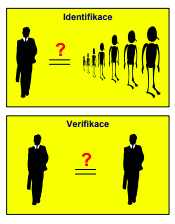
\includegraphics[width=150]{obrazky-figures/identifver.png}
    \caption{Rozdíl mezi identifikací a verifikací, převzato z \cite{Drahansky}}
    \label{fig:markants}
\end{figure}



\section{Biometrické systémy}
Biometrické systémy dělíme do dvou základních kategorií\cite{Drahansky}:
\begin{itemize}
    \item Registrační modul - Zde je zaregistrována biometrická informace (tzv. biometrický markant) a je uložena do databáze.
    \item Verifikační modul - Zde je zaregistrována biometrická informace podobně jako u registračního modulu, ale výsledek není uložen do databáze, nýbrž jsou data z databáze načítána, aby se extrahovaný biometrický markant mohl porovnat s daty v databázi. 
\end{itemize}

\begin{figure}[htbp]
    \centering
    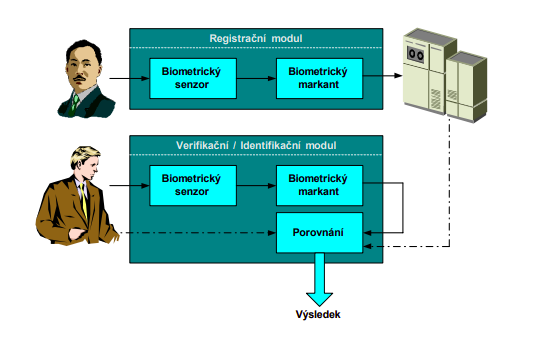
\includegraphics[width=340]{obrazky-figures/biosystem.png}
    \caption{Znázornění biometrického systému, převzato z \cite{Drahansky}}
    \label{fig:markants}
\end{figure}

\chapter{Detekce otisků prstů}
\section{Historie}
Lidské otisky prstů byly objeveny na velkém počtu archeologických artefaktů a historických předmětech. I když tyto nálezy dokazují, že lidé v té době byli vědomi unikátnosti otisků prstů, až v 16. století byla objevena první vědecká technika v jejich výzkumu. V roce 1864 anglický vědec Nehemiah Grew publikoval první vědeckou studii o hřebenech, rýhách a pórech v struktuře otisku prstu.

První detailní popis struktury otisků prstů byl předveden Mayerem v roce 1788. Purkinje pak roku 1823 vytvořil první klasifikační schéma, ve kterém otisky prstů rozdělil do devíti kategorií na základě konfigurace hřebenů.\cite{Maltoni2009}

\section{Zákony daktyloskopie}
Byly zavedeny tyto daktyloskopické zákony\cite{Drahansky}:
\begin{itemize}
    \item Struktura papilárních linií je unikátní pro každého jedince.
    \item Vzor tvořený papilárními liniemi je pro každého jedince během života relativně neměnný.
    \item Obnova papilárních liní probíhá dorůstáním kůže na povrchu prstů. Mohou být pozměněny pouze pokud se poškodí nebo odstranní epidermální vrstva kůže. Poté již nemůže docházet k obnově.
    \item Konfigurační typy se mohou individuálně měnit, jedná se však o malé změny, které leží v tolerančních limitech a umožňují tak systematickou klasifikaci.
\end{itemize}

\section{Struktura otisku prstu}
Otisk prstu je tvořen vzorem papilárních linií. Výška papilárních je v rozmezí 0,1 - 0,4 mm a šířka v rozmezí 0,2 - 0,5 mm.\cite{Drahansky} Průběhy papilárních linií jsou jedinečné pro každého člověka. S přibývajícím věkem se mění rozměry plošek prstů či dlaní, avšak struktura papilárních linií zůstává stejná.

Nejvýznamější atributy papilárních liníí se vyvýjí již v nitroděložní části života. Konečná podoba papilárních linií je u dítěte již v 6. - 7. měsíci nitroděložního vývoje.\cite{DrahanskyBrezinova}

Otisky prstů dělíme na základní tři druhy:\cite{Drahansky}
\begin{itemize}
\item Válený otisk (barvený, rolovaný)
\item Píchaný otisk (živý)
\item Latentní otisk (skrytý)
\end{itemize}

\begin{figure}[htbp]
    \centering
    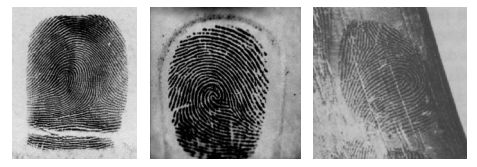
\includegraphics[width=340]{obrazky-figures/druhyotisk.png}
    \caption{Válený, píchaný a latentní otisk prstu, převzato z \cite{Drahansky}}
    \label{fig:druhyotisk}
\end{figure}

\section{Typy senzorů}
Nejdůležitějším částí detekce je senzor, který zaznamenává výsledný otisk prstu. Řadíme je do těchto základních kategorií:
\begin{itemize}
\item Optické senzory - Využívají jednoduchý zdroj světla (LED), které osvětlí plochu prstu.\cite{Drahansky} Nejvíce používaným zástupcem optických senzorů je senzor FTIR. Prst se při snímání dotýká skleněného nebo plastového hranolu. Při dotyku jsou hřebeny papilárních linií v kontaktu s povrchem snímače, ale údolí jsou vzdálena. Světlo pocházející z hranolu dopadá na prst a je odraženo údolími papilárních liníí nebo náhodně pohlceno hřebeny. Ve výsledném obrazu jsou pak hřebeny tmavá místa a údolí světlá místa. FTIR snímače dokáží snímat 3D otisk prstu a tak dokáží detekovat i zfalšované otisky prstu, které například pocházejí z fotografie. \cite{Maltoni2009}

\begin{figure}[htbp]
    \centering
    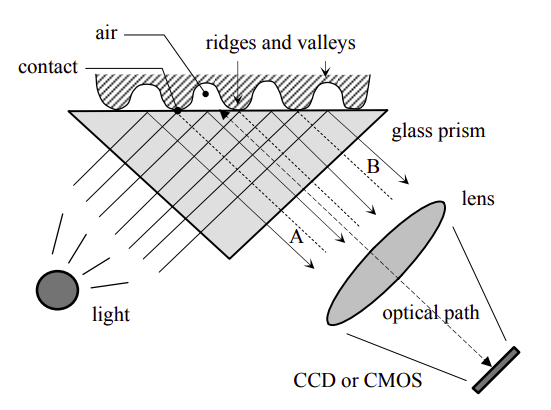
\includegraphics[width=250]{obrazky-figures/ftiredit.png}
    \caption{Senzor FTIR, převzato z \cite{Maltoni2009}}
    \label{fig:ftir}
\end{figure}

\item Kapacitní senzory - Jsou složeny z matice malých vodivých plošek, na níž je napařena vrstva nevodivého oxidu křemičitého.\cite{Drahansky} Mezi povrchem prstu a každou z plošek (mikrokapacitorů) v čipu vzniká malý elektrický náboj. Při skládání výsledného otisku prstu je důležitá vzdálenost mezi povrchem otisku prstu a mikrokapacitorem. Hřebeny a údolí papilárních linií otisku prstu mají jinou vzdálenost od mikrokapacitoru, tudíž i odlišnou intenzitu ve výsledném obraze. Stejně jako u senzoru FTIR nemůže tato technologie být zneužita útočníkem při předložení fotografie. Jsou zde totiž měřeny vzdálenosti a pouze trojrozměrný povrch může být nasnímán.\cite{Maltoni2009}

\begin{figure}[htbp]
    \centering
    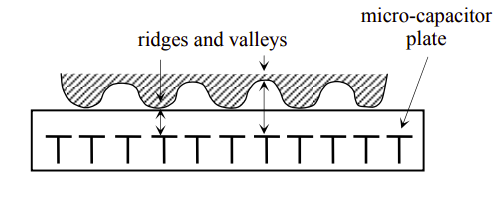
\includegraphics[width=300]{obrazky-figures/kapacit.png}
    \caption{Kapacitní senzor, převzato z \cite{Maltoni2009}}
    \label{fig:electro}
\end{figure}
\item Ultrazvukové senzory - Jsou založeny na posílání akustického signálu prstu a zachytávání odraženého signálu. Odražený signál je použit na výpočet hloubky obrazu a struktury papilárních linií. Senzor se skládá z vysílače a příjimače. Vysílač generuje krátké zvukové pulsy a příjímač detekuje odpověď po odražení těchto akustických pulsů od povrchu prstu. Senzor je schopný detekovat strukturu otisku prstu i např. přes tenké rukavice, stejně jako si dokáže poradit s nečistotami i mastnotou.\cite{Maltoni2009}

\begin{figure}[htbp]
    \centering
    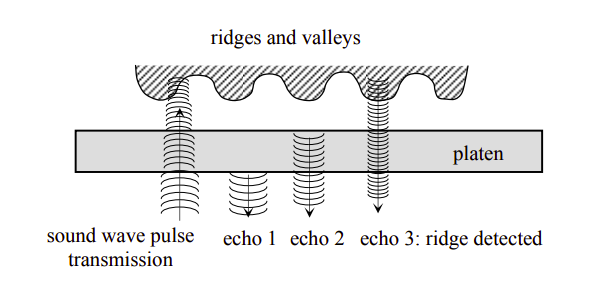
\includegraphics[width=300]{obrazky-figures/ultrasound.png}
    \caption{Ultrazvukový senzor, převzato z \cite{Maltoni2009}}
    \label{fig:ultrasound}
\end{figure}
\item Elektrooptické senzory - Tyto snímače jsou složeny ze dvou vrstev. První dokáže emitovat světlo, pokud je polarizována správným nápětím. Druhá vrstva úzce spolupracuje s první, zpracovává emitované světlo a vytváří finální digitální obraz.\cite{Maltoni2009}

\begin{figure}[htbp]
    \centering
    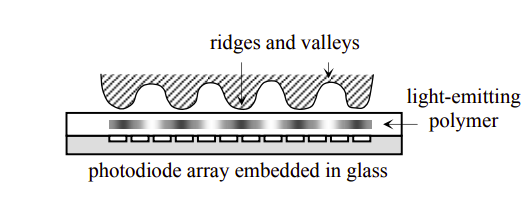
\includegraphics[width=300]{obrazky-figures/electro.png}
    \caption{Elektrooptický senzor, převzato z \cite{Maltoni2009}}
    \label{fig:electro}
\end{figure}
\item Tlakový senzor - Je vytvořen z materiálu citlivého na mechanické namáhání, při kterém generuje elektrický signál. Velikost elektrického signálu závisí na tlaku, který vyvíjí prst na povrch senzoru. Hřebeny a údolí papilárních linií jsou v jiných vzdálenost od povrchu snímače, proto produkují jinou hodnotu elektrického signálu.\cite{Maltoni2009}
\item Termický senzor - Senzor využívá pyroelektrický materiál, který generuje elektrický náboj na základě teplotních rozdílů. Je založen na skutečnosti, že hřebeny v kontaktu s povrchem senzoru produkují jinou teplotu jak údolí, které jsou vzdálenější od povrchu snímače. Senzor je obvykle předehřán na vyšší teplotu, aby se zvýšila odlišnost mezi povrchem zařízení a hřebeny linií.\cite{Maltoni2009}
\end{itemize}

\section{Základní druhy markantů}
Otisk prstu obsahuje útvary, které tvoří papilární linie - markanty. Mezi důležité markanty pro moji práci patří:
\begin{itemize}
    \item Ukončení (Line Ending)
    \item Jednoduchá vidlička (Simple Bifurcation)
    \item Dvojitá vidlička (Double Bifurcation)
    \item Trojitá vidlička (Triple Bifurcation)
    \item Hák (Hook)
    \item Křížení (Crossing)
    \item Boční kontakt (Side Contact)
    \item Bod (Point)
    \item Interval (Interval)
    \item Jednoduchá smyčka (Single Whorl)
    \item Dvojitá smyčka (Double Whorl)
    \item Jednoduchý most (Single Bridge)
    \item Dvojitý most (Twin Bridge)
    \item Průsečná linie (Through Line)
\end{itemize}

\begin{figure}[htbp]
    \centering
    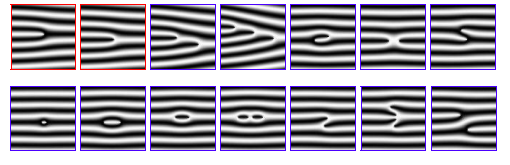
\includegraphics[width=250]{obrazky-figures/markants.png}
    \caption{Základní typy markantů ve vyjmenovaném pořadí, převzato z \cite{Drahansky}}
    \label{fig:markants}
\end{figure}

U přístupových systémů se však využívá pouze ukončení (Line Ending) a vidličky (Bifuraction).\cite{Drahansky}

\section{Třídy otisků prstů}
Otisky prstů můžeme na základě charakteristických znaků rozdělit do následujících kategorií:\cite{Drahansky}
\begin{itemize}
    \item Oblouk (Arch)
    \item Klenutý oblouk (Tended Arch)
    \item Spirála / závit (Whorl)
    \item Levá smyčka (Left Loop)
    \item Pravá smyčka (Right Loop)
    \item Dvojitá smyčka (Twin Loop)
\end{itemize}

\begin{figure}[htbp]
    \centering
    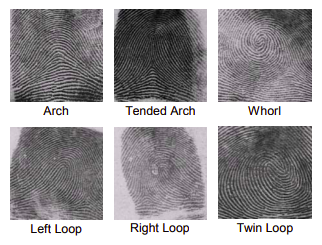
\includegraphics[width=300]{obrazky-figures/classes.png}
    \caption{Třídy otisků prstů, převzato z \cite{Drahansky}}
    \label{fig:classes}
\end{figure}

\section{Falšování otisků prstů}
Falešné biometrické reprezentace jsou obecně velkým nebezpečím, protože umožňují vydávat se zločinci za někoho jiného a tím narušit soukromí a bezpečnost jedince. Abnormální otisky prstů dělíme do dvou kategorií:
\begin{itemize}
    \item Falešné otisky prstů
    \item Pozměněné otisky prstů
\end{itemize}
Falešný otisk prstu reprezentuje repliku skutečného otisku prstu vyrobeného softwarově nebo z materiálů jako je želatina, silikon nebo latex. Biometrické zařízení se musí rozhodnout, zda otisk je živý nebo falešný. Tato procedura se nazývá detekce živosti.
Pozměněné otisky prstů jsou skutečné, avšak jejich struktura je změněna. Otisky mohou být neúplné, pokřivené. Důvodem poškození otisku mohou být nemoci kůže, např. pořezání, popálenina, poleptání silnými chemikáliemi, transplantace kůže a různé kožní nemoci.\cite{Petrovici}
\section{Známé metody pro analýzu živosti otisku prstu}
Algoritmů pro detekci živosti otisku prstu byla objevena ve studiích celá řada. Některé z nich jsou:\cite{AbhiskekStudy}
\begin{itemize}
    \item Pomocí použití vlastnosti elasticity lidské kůže.
    \item Umístění senzoru na zachytávání pachu vedle senzoru pro detekci otisku prstu. Senzor pachu zaznamenával výsledný signál a byl tak schopen rozpoznat lidskou kůži od syntetických materiálů, jako např. latex, silikon nebo želatina.
    \item Kombinace statických vlastností při detekci živosti, bylo pracováno s histogramem, tloušťkou hřebenů papilárních linií, signálem detekovaným z hřebenů nebo hodnota výkonnového frekvenčního spektra.
    
\end{itemize}

Přesnost analýzy živosti $a$ můžeme spočítat na základě vzorce:
$a = \frac{C}{N}$, kde $C$ je počet správných rozhodnutí (klasifikace živého otisku prstu jako "živého" a falešného otisku prstu jako "falešného") a $N$ je počet všech rozhodnutí.\cite{GottschlichStudy}


\chapter{Algoritmy pro analýzu živosti otisků prstů}
Před samotnou implementací hlavních algoritmů bylo potřeba otisk prstu upravit, udělat prvotní předzpracování. V této kapitole na základě vzorců a pravidel jednotlivé algoritmy popíši. V letním semestru plánuji používané algoritmy a postupy rozšířit. 
\section{Převedení na normalizovaný obraz}
Po načtení obrazu bylo potřeba obraz převést na šedotonový. Poté byla provedena normalizace obrazu. Normalizace je proces, při kterém je upraven rozsah hodnot intenzity pixelu. Základem je zvýšit dynamický rozsah šedotónového jasu, u otisků prstů tento algoritmus nemění ostrost hřebenů a údolí papilárních linií. Hlavním účelem je minimalizovat změny šedo-úrovňových hodnot podél hřebenů a údolí. 

\begin{figure}[htbp]
  \begin{minipage}[b]{0.5\linewidth}
    \centering
    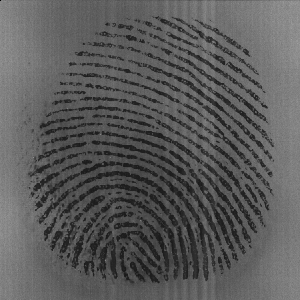
\includegraphics[width=\linewidth]{obrazky-figures/102_1.png}
    \caption{Vstupní obraz}
    \label{fig:origimg}
  \end{minipage}
  \hspace{0.5cm}
  \begin{minipage}[b]{0.5\linewidth}
    \centering
    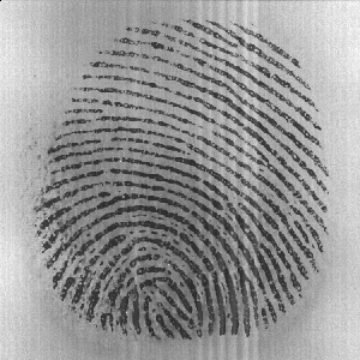
\includegraphics[width=\linewidth]{obrazky-figures/norm_img.png}
    \caption{Normalizovaný obraz}
    \label{fig:normimg}
  \end{minipage}
\end{figure}



\section{Prahování}
Při prahování jsou světlé objekty odděleny od tmavých pomocí zadaných konstantních prahů. Tento algoritmus je nutno použít před samotnou segmentací obrazu pomocí morfologických metod.

\begin{figure}[htbp]
  \begin{minipage}[b]{0.5\linewidth}
    \centering
    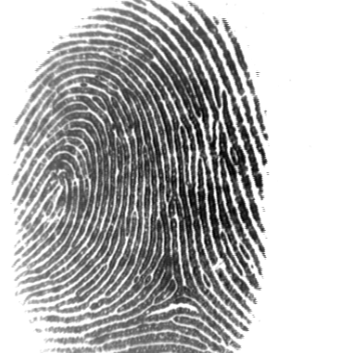
\includegraphics[width=180]{obrazky-figures/104_7norm.png}
    \caption{Normalizovaný obraz}
    \label{fig:origimg}
  \end{minipage}
  \hspace{0.5cm}
  \begin{minipage}[b]{0.5\linewidth}
    \centering
    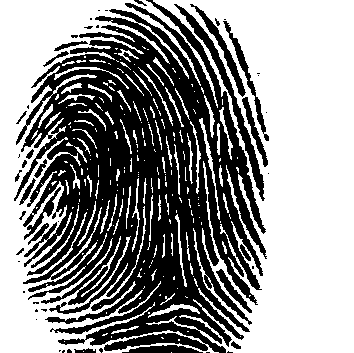
\includegraphics[width=180]{obrazky-figures/tresh104.png}
    \caption{Obraz po aplikaci prahování}
    \label{fig:normimg}
  \end{minipage}
\end{figure}
\section{Segmentace}
Při segmentaci vybereme z vstupního obrazu pouze otisk prstu, což nám napomáhá eliminovat pozadí obrazu. Bylo využito morfologického otevření - kombinace eroze a následné diletace obrazu.

Morfologické operace se používají obvykle na úpravu binárního obrazu. Potřebují dva vstupy - náš vstupní obraz a jádro.\cite{OpenCVMorphology} Tyto operace se používají často na obrazové předzpracování - odstraňují šum a zjednodušují tvary objektů. Eroze je morfologickou operací, která je užitečná pro odstranění malých bílých částí v obraze. Diltace je opakem eroze a použivá se k zaplnění mezer.\cite{ExerciseMorphology}

Papilární linie jsou odděleny po vyprahování úzkými místy a tento algoritmus má za cíl úzká místa spojit a vytvořit tak masku, která bude určovat pozici otisku prstu v obrazu. Struktura objektu se tedy při vzniku masky zjednodušší. Výsledná maska je následně aplikována na normalizovaný obraz a je tedy vybrána pouze část obrazu, která obsahuje otisk prstu, pozadí zůstává bílé.

\begin{figure}[htbp]
  \begin{minipage}[b]{0.3\linewidth}
    \centering
    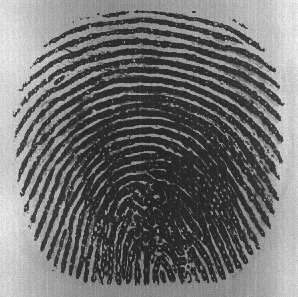
\includegraphics[width=\linewidth]{obrazky-figures/105_5norm.png}
    \caption{Vstupní normalizovaný obraz}
    \label{fig:normimg105}
  \end{minipage}
  \hspace{0.3cm}
  \begin{minipage}[b]{0.3\linewidth}
    \centering
    
\includegraphics[width=\linewidth]{obrazky-figures/105_5mask.png}
    \caption{Získaná maska}
    \label{fig:mask}
  \end{minipage}
  \hspace{0.3cm}
    \begin{minipage}[b]{0.3\linewidth}
    \centering
    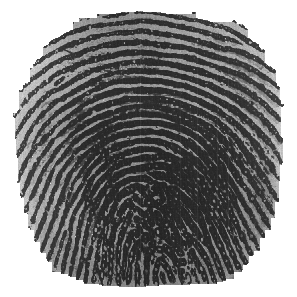
\includegraphics[width=\linewidth]{obrazky-figures/105_5segment.png}
    \caption{Výsledný segmentovaný obraz}
    \label{fig:mask}
  \end{minipage}
\end{figure}

\section{Ztenčování linií}
Pro extrakci markantů (ukončení a vidličky) je potřeba ztenčit papilární linie otisku prstů. Pro ztenčení bylo znovu využito morfologických operací. V každé iteraci algoritmu je znovu provedena eroze obrazu.
Známým postupem pro vytvoření morfologické kostry je Lantuéjoulova formule:\cite{WikipediaSkeleton}\\\\
Pro diskrétní binární obraz $X$$\subset$$\mathds{Z}^2$, skeleton $S(X)$ je sjednocením podmnožin koster ${S_n(X)},$\\$ n = 0,1,..,N$, kde:
$$S_n(X) = (X \ominus nB) - (X \ominus nB) \circ B$$ Symboly $\ominus$ a $\circ$ jsou morfologická eroze a otevření. 

\begin{figure}[htbp]
  \begin{minipage}[b]{0.5\linewidth}
    \centering
    
\includegraphics[width=\linewidth]{obrazky-figures/SG_LLnorm.png}
    \caption{Vstupní normalizovaný a segmentovaný obraz}
    \label{fig:origimg}
  \end{minipage}
  \hspace{0.5cm}
  \begin{minipage}[b]{0.5\linewidth}
    \centering
    
\includegraphics[width=\linewidth]{obrazky-figures/SG_LLthin.png}
    \caption{Obraz se ztenčenými papilárními liniemi}
    \label{fig:normimg}
  \end{minipage}
\end{figure}
\section{Extrakce ukončení a vidličky}
Extrakce těchto nejdůležitějších markantů v otisku prstu probíhá po normalizaci, segmentaci a ztenčení obrazu. Předchozí práce ukázala, že úroveň jasu v šedotónovém obrazu je náhodnou u živých otisků prstů, ale má sklon být buď uniformní nebo periodická u falešných otisků prstů. Stejná myšlenka je pak použita u místní analýzy textury otisku prstu. Z tohoto důvodu počet hřebenů ukončení papilárních linií u živých otisků prstů má tendenci dosahovat k větším číslům, jak u falešných otisků prstů. Proto je očividné, že tato metoda může být efektivní vlastností, jak odlišit živé otisky prstů od falešných.\cite{AbhiskekStudy}

\begin{figure}[htbp]
    \centering
    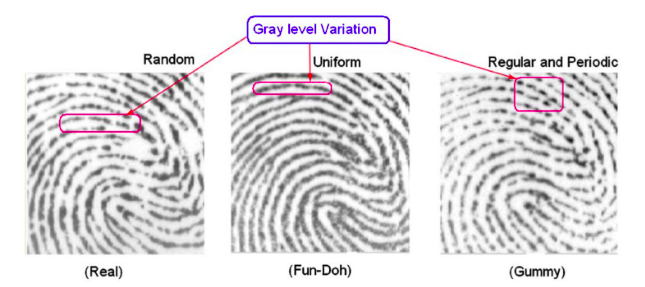
\includegraphics[width=400]{obrazky-figures/graylevel.png}
    \caption{Ukázka změn úrovně šedotónového jasu u živých otisků prstů v porovnání s falešnými otisky z syntetických materiálů, převzato z \cite{AbhiskekStudy}}
    \label{fig:graylevel}
\end{figure}

Pro extrakci ukončení i vidličky bylo použito okna o velikosti 3x3 pixely. U každého pixelu pak bylo na základě tohoto okna ve středu s procházeným pixelem zjištěno, jaké hodnoty mají jeho sousedé a tento prostřední centrální pixel. 

Hledání ukončení papilárních linií probíhalo za pomocí následujícího okna:

\begin{figure}[htbp]
    \centering
    
\includegraphics[width=350]{obrazky-figures/windowridge.png}
    \caption{Okno o velikosti 9 pixelů pro extrakci ukončení, převzato z \cite{BansalStudy}}
    \label{fig:ridgewindow}
\end{figure}





\section{Extrakce orientovaného pole}
Tento algoritmus z detekovaného otisku prstu vytvoří orientovanou mapu. Algoritmus postupuje následovně:\\
1. Rozdělte normalizovaný obraz $G$ na bloky o velikosti $w$ x $w$.\\
2. Spočítejte gradienty $\delta_x$$(i, j)$ a $\delta_y$$(i, j)$ v každém pixelu obrazu. \\
2. Odhadněte místní orientaci každého bloku se středem v pixelu $(i, j)$ pomocí těchto rovnic:
$$V_x(i, j) = \sum_{u=i-\frac{w}{2}}^{i+\frac{w}{2}}\sum_{v=j-\frac{w}{2}}^{j+\frac{w}{2}} 2\delta_x(u,v)\delta_y(u,v)$$
$$V_y(i, j) = \sum_{u=i-\frac{w}{2}}^{i+\frac{w}{2}}\sum_{v=j-\frac{w}{2}}^{j+\frac{w}{2}} \delta_x^2(u,v) - \delta_y^2(u,v)$$
$$\theta(i, j) = \frac{1}{2}\tan^{-1}(\frac{V_y(i,j)}{V_x(i, j)}$$
3. Spočítejte magnitudu:
$$V(i,j) = \sqrt{V_x(i,j)^2 + V_y(i,j)^2}$$
4. Převeďte orientovaný obraz na souvislé pole vektorů pomocí rovnic:
$$\Phi_x(i,j) = V(i,j)\cos{2\theta(i,j)}$$
$$\Phi_y(i,j) = V(i,j)\sin{2\theta(i,j)}$$
5. Vypočítejte výsledný úhel se středem v pixelu $(i, j)$:
$$O(i, j) = \frac{1}{2}\tan^{-1}(\frac{\Phi_y(i,j)}{\Phi_x(i, j)}$$
Výsledné vykreslení orientovaných úseček probíhá následovně:\\
6. Vypočítejte počáteční body $(x_0,y_0)$ orientované úsečky:\\
$$x_0 = i + \frac{w}{2}$$
$$y_0 = j + \frac{w}{2}$$
7. Vypočítejte koncové body $(x_1,y_1)$ orientované úsečky:\\
$$r = \frac{w}{2}$$
$$x_1 = r * \cos({O(i,j)})+ x_0$$
$$y_1 = r * \sin({O(i,j)})+ y_0$$
8. Sestavte výsledné rovnice orientovaných úseček. Vypočtený úhel je kolmý směrem k hřebenům papilárních linií:\\
$$x_1 = r * cos(O(i,j)- \frac{\pi}{2}) + x_0$$
$$y_1 = r * sin(O(i,j)- \frac{\pi}{2}) + y_0$$

\begin{figure}[htbp]
  \begin{minipage}[b]{0.5\linewidth}
    \centering
    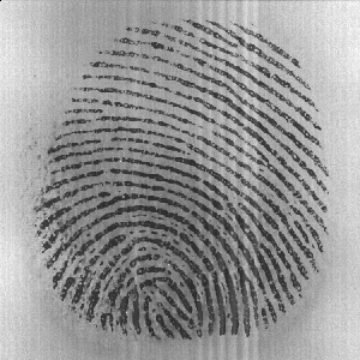
\includegraphics[width=175]{obrazky-figures/norm_img.png}
    \caption{Normalizovaný a segmentovaný obraz}
    \label{fig:origimg}
  \end{minipage}
  \hspace{0.5cm}
  \begin{minipage}[b]{0.5\linewidth}
    \centering
    
\includegraphics[width=190]{obrazky-figures/orient.png}
    \caption{Orientované pole obrazu}
    \label{fig:normimg}
  \end{minipage}
\end{figure}



\section{Lokální binární vzor}
Lokální binární vzor byl hlavním algoritmem, s jehož výstupy budu dále při práci pracovat. Jedná se o efektivní algoritmus, který se používá pro analýzu textury objektů.  Algoritmus je užitečný pro informace o změnách intenzity mezi jednotlivými pixely obrázku a jejich sousedy. Kalkulace lokálního binárního vzoru vypadá následovně:\cite{GaikwadStudy}

$$LBP(x_c,y_c) = \sum_{n=0}^{7}2^n(I_n-I(x_c,y_c)),$$
kde $I_n$ jsou hodnoty sousedních pixelů a a $I(x_c,y_c)$ hodnota středového pixelu, $n$ je index souseda.\\\\
Postup algoritmu je následující:\\
1. Pro každý pixel je zjištěno okno 3x3 pixely, kde námi procházený pixel x je středem, středem s 8 sousedy.\\
2. Pro každý pixel v 3x3 okně je spočítána nová hodnota na základě tohoto pravidla - Pokud je hodnota zjišťovaného pixelu větší nebo rovna hodnotě středového pixelu, pak je novou hodnotou zjišťovaného pixelu 1, jinak 0.\\
3. Po spočítání nových hodnot celého 3x3 okna je spočítána nová binární hodnota středového pixelu.\\

\begin{figure}[htbp]
    \centering
    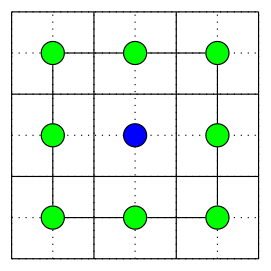
\includegraphics[width=120]{obrazky-figures/lbpn.png}
    \caption{Okno o velikosti 9 pixelů se středovým pixelem a jeho sousedy pro analýzu lokálního binárního vzoru, převzato z \cite{GragnanielloStudy}}
    \label{fig:localne}
\end{figure}

\begin{figure}[htbp]
    \centering
    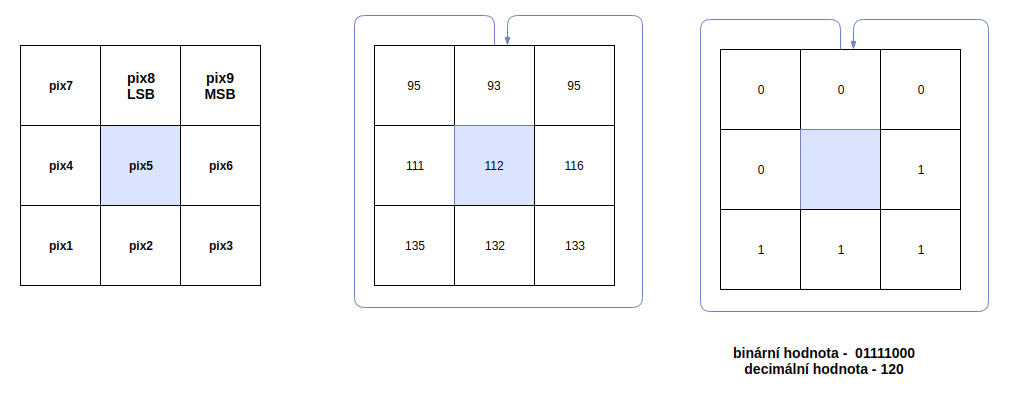
\includegraphics[width=351]{obrazky-figures/lbpprincip.png}
    \caption{Princip výpočtu lokálního binárního vzoru, upraveno s využitím \cite{GaikwadStudy}}
    \label{fig:lbpprincip}
\end{figure}

 Nyní bylo potřeba vyextrahovat pro lokální binární vzor informace, na základě kterých by se dala detekovat problematika živosti otisku prstu. První informací, kterou jsem si z nového obrazu vyextrahovala byl jeho histogram. Histogramy se zvláště ve středových hodnotách podstatně liší. Svoji hypotézu jsem otestovala na základě porovnání sum hodnot histogramů v jejich druhém a třetím kvadrantu. Na základě prahu jsem pak mohla rozhodnout, zda je otisk prstu živý nebo falešný.
 
 Hypotéza byla otestována na třech databázích - dvou obsahující živé otisky prstu a jedné obsahující falešné otisky prstů. Celkem bylo pracováno se 140 snímky. Při výpočtu přesnosti budu využívat již zmiňovaný vzorec:\\
 $$a = \frac{C}{N}$$
 Do vzorce dosadíme:\\
  $$a = \frac{122}{140} = 87,14\%$$
 
 Analýzou lokálního binárního vzoru pro detekci živosti a  dalšími algoritmy se budu dále zabívat v letním semestru.
 
 \begin{figure}[htbp]
  \begin{minipage}[b]{0.3\linewidth}
    \centering
    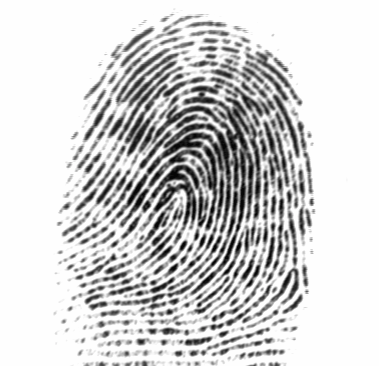
\includegraphics[width=\linewidth]{obrazky-figures/db3.png}
    \caption{Snímek z databáze DB1\_B (University at Bologna)}
    \label{fig:normimg105}
  \end{minipage}
  \hspace{0.3cm}
  \begin{minipage}[b]{0.3\linewidth}
    \centering
    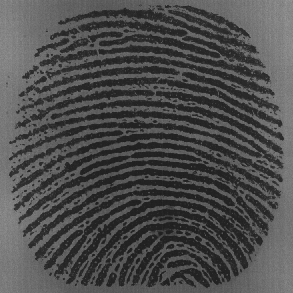
\includegraphics[width=\linewidth]{obrazky-figures/db2.png}
    \caption{Snímek z databáze DB3\_B (University at Bologna)}
    \label{fig:mask}
  \end{minipage}
  \hspace{0.3cm}
    \begin{minipage}[b]{0.3\linewidth}
    \centering
    
\includegraphics[width=100]{obrazky-figures/db1.png}
    \caption{Snímek z obdržené databáze falešných otisků prstů}
    \label{fig:mask}
  \end{minipage}
\end{figure}

\begin{figure}[htbp]
  \begin{minipage}[b]{0.5\linewidth}
    \centering
    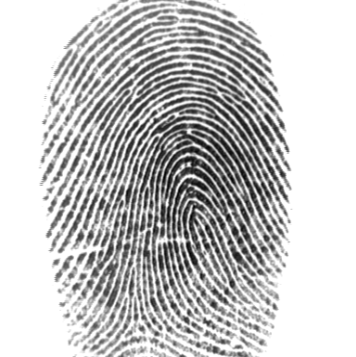
\includegraphics[width=200]{obrazky-figures/107_7.png}
    \caption{Vstupní normalizovaný a segmentovaný obraz živého otisku prstu}
    \label{fig:origimg107}
  \end{minipage}
  \hspace{0.5cm}
  \begin{minipage}[b]{0.5\linewidth}
    \centering
    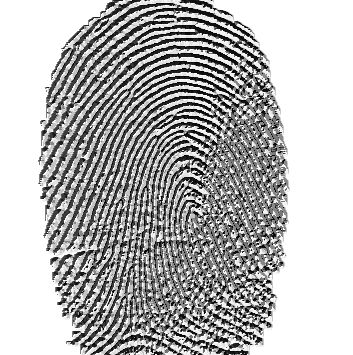
\includegraphics[width=200]{obrazky-figures/107_7lbp.png}
    \caption{Výsledek aplikace lokálního binárního vzoru}
    \label{fig:lbplive}
  \end{minipage}
\end{figure}

\begin{figure}[htbp]
  \begin{minipage}[b]{0.5\linewidth}
    \centering
    
\includegraphics[width=200]{obrazky-figures/SG_LLnorm.png}
    \caption{Vstupní normalizovaný a segmentovaný obraz falešného otisku prstu}
    \label{fig:origimgSGLL}
  \end{minipage}
  \hspace{0.5cm}
  \begin{minipage}[b]{0.5\linewidth}
    \centering
    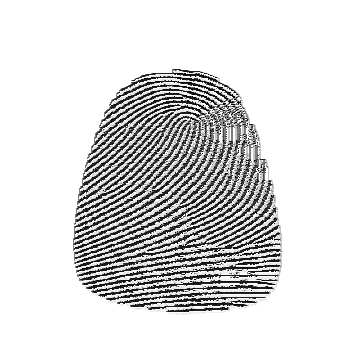
\includegraphics[width=200]{obrazky-figures/SDLBP.png}
    \caption{Výsledek aplikace lokálního binárního vzoru}
    \label{fig:lbpfake}
  \end{minipage}
\end{figure}


\begin{figure}[htbp]
    \centering
    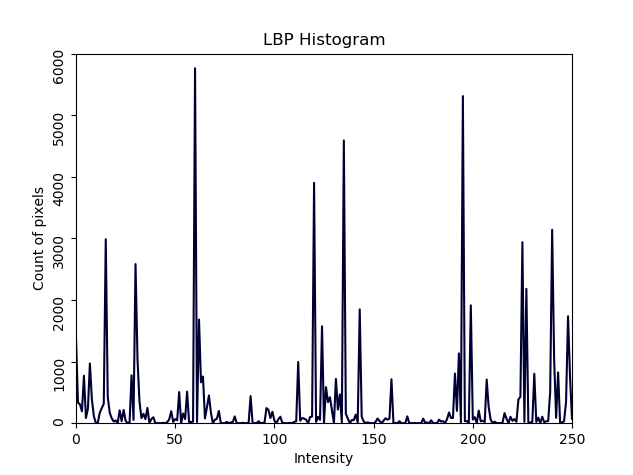
\includegraphics[width=300]{obrazky-figures/histogramlive.png}
    \caption{Histogram pro výsledek lokálního binárního vzoru pro živý otisk prstu}
    \label{fig:lbphistlive}
\end{figure}






\begin{figure}[htbp]
    \centering
    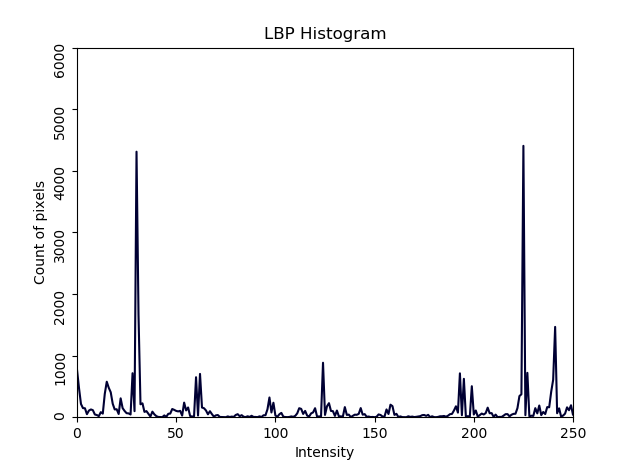
\includegraphics[width=300]{obrazky-figures/histfake.png}
    \caption{Histogram pro výsledek lokálního binárního vzoru pro falešný otisk prstu}
    \label{fig:lbphistfake}
\end{figure}








\label{citace}



\chapter{Závěr}
V průběhu zimního semestru jsem se v rámci povinného předmětu Semestrální projekt (ITT) začala seznamovat s tématem detekce živosti otisků prstů. Nastudovala jsem odborné články a literaturu, začala jsem pracovat na algoritmech pro předzpracování obrazu (normalizace, prahování, ztenčování linií, extrakce orientovaného pole, extrakce markantů). Začala jsem implementovat hlavní algoritmus pro detekci živosti - lokální binární vzor. V průběhu letního semestru budu svoji práci dále rozšiřovat a zdokonalovat, chci provést výzkum nejen softwarově generovaných otisků prstů, ale i otisků prstů z různých syntetických materiálů. Plánuji navštívit laboratoř a získat snímky syntetických otisků prstů z senzoru. Svoji detekci živosti prstu chci vedle extrakce markantů a lokálního binárního vzoru rozšířit také o práci s vlnovou délkou. Jednotlivé algoritmy poté porovnám na základě přesnosti či rychlosti zpracování. 

\label{zaver}



  \fi
  
  % Kompilace po částech (viz výše, nutno odkomentovat)
  % Compilation piecewise (see above, it is necessary to uncomment it)
  %\subfile{projekt-01-uvod-introduction}
  % ...
  %\subfile{chapters/projekt-05-conclusion}


  % Pouzita literatura / Bibliography
  % ----------------------------------------------
\ifslovak
  \makeatletter
  \def\@openbib@code{\addcontentsline{toc}{chapter}{Literatúra}}
  \makeatother
  \bibliographystyle{bib-styles/Pysny/skplain}
\else
  \ifczech
    \makeatletter
    \def\@openbib@code{\addcontentsline{toc}{chapter}{Literatura}}
    \makeatother
    \bibliographystyle{bib-styles/Pysny/czplain}
  \else 
    \makeatletter
    \def\@openbib@code{\addcontentsline{toc}{chapter}{Bibliography}}
    \makeatother
    \bibliographystyle{bib-styles/Pysny/enplain}
  %  \bibliographystyle{alpha}
  \fi
\fi
  \begin{flushleft}
  \bibliography{projekt-20-literatura-bibliography}
  \end{flushleft}

  % vynechani stranky v oboustrannem rezimu
  % Skip the page in the two-sided mode
  \iftwoside
    \cleardoublepage
  \fi

  % Prilohy / Appendices
  % ---------------------------------------------
  \appendix
\ifczech
  \renewcommand{\appendixpagename}{Přílohy}
  \renewcommand{\appendixtocname}{Přílohy}
  \renewcommand{\appendixname}{Příloha}
\fi
\ifslovak
  \renewcommand{\appendixpagename}{Prílohy}
  \renewcommand{\appendixtocname}{Prílohy}
  \renewcommand{\appendixname}{Príloha}
\fi
%  \appendixpage

% vynechani stranky v oboustrannem rezimu
% Skip the page in the two-sided mode
%\iftwoside
%  \cleardoublepage
%\fi
  
\ifslovak
%  \section*{Zoznam príloh}
%  \addcontentsline{toc}{section}{Zoznam príloh}
\else
  \ifczech
%    \section*{Seznam příloh}
%    \addcontentsline{toc}{section}{Seznam příloh}
  \else
%    \section*{List of Appendices}
%    \addcontentsline{toc}{section}{List of Appendices}
  \fi
\fi
  \startcontents[chapters]
  \setlength{\parskip}{0pt} 
  % seznam příloh / list of appendices
  % \printcontents[chapters]{l}{0}{\setcounter{tocdepth}{2}}
  
  \ifODSAZ
    \setlength{\parskip}{0.5\bigskipamount}
  \else
    \setlength{\parskip}{0pt}
  \fi
  
  % vynechani stranky v oboustrannem rezimu
  \iftwoside
    \cleardoublepage
  \fi
  
  % Přílohy / Appendices
  \ifenglish
    \input{projekt-30-prilohy-appendices-en}
  \else
    % Tento soubor nahraďte vlastním souborem s přílohami (nadpisy níže jsou pouze pro příklad)

% Umístění obsahu paměťového média do příloh je vhodné konzultovat s vedoucím
%\chapter{Obsah přiloženého paměťového média}

%\chapter{Manuál}

%\chapter{Konfigurační soubor}

%\chapter{RelaxNG Schéma konfiguračního souboru}

%\chapter{Plakát}


  \fi
  
  % Kompilace po částech (viz výše, nutno odkomentovat)
  % Compilation piecewise (see above, it is necessary to uncomment it)
  %\subfile{projekt-30-prilohy-appendices}
  
\end{document}
